\section{Results}



\subsection{Mechanism}
\subsubsection{Experiment 1: Update Frequency of Trending Stories}
To measure the system-wide update frequency, we ran the automated data collection every two minutes over a 24-hour period, closing the app and erasing the cache folder each time the simulator collected stories. The average time between updates -- either a change in the order of stories or the addition of a new story -- was 20 minutes (min=6 mins, max=61 mins, median=17 mins, sd=11 mins). We ran the user-specific update frequency experiment during the same time (closing the app but not removing cache and user profile files) and found identical update times. However, when the simulator kept the app open in between checking for new stories, the Trending Stories section did not change for the full 24 hours.
%if the simulator did not go to the home screen or close the app in some way between data points, the Trending Stories section did not change for the full 24 hours.

%changed twice within fifteen minutes,  

\begin{comment}
\pgfplotstableread[row sep=\\,col sep=&]{
interval & pct \\
0--5     & 0 \\
5--10     & 7.6923077 \\
10--15    & 38.4615385\\
15--20   & 23.0769231 \\
20--25   & 3.8461538 \\
25--30   & 7.6923077 \\
30--35   & 7.6923077 \\
35+      & 11.5384615 \\
    }\mydata
    
    
    
\begin{figure}[t]
\begin{center}
\begin{tikzpicture}
    \begin{axis}[
            ybar,
            symbolic x coords={0--5,5--10,10--15,15--20,20--25,25--30,30--35,35+},
            ymajorgrids=true,
nodes near coords=\pgfmathprintnumber{\pgfplotspointmeta}\%,
every node near coord/.append style={font=\scriptsize},
nodes near coords style={/pgf/number format/.cd,fixed zerofill,precision=1},
            xtick=data,
        ]
        \addplot[fill=gray,draw=none] table[x=interval,y=pct]{\mydata};
    \end{axis}
\end{tikzpicture}
\end{center}
\caption{Relative distribution of minutes between updates}\label{minutes-between-updates}
\end{figure}
\end{comment}

\subsubsection{Experiment 2: Localization of Trending Stories}
We ran our experiment to test for localization on two occasions, finding no variation in trending stories that could be attributed to differences in location. In other words, at all 50 experimental locations, the list of Trending Stories in the experimental location matched the list of Trending Stories in the control location, thus showing no evidence of location-based content adaptation. The experiment took about an hour and a half to run.

\subsubsection{Experiment 3: Personalization of Trending Stories}
We collected synchronized screenshots on three occasions, yielding 28 data points in the first experiment, 32 in the second, and 29 in the third for a total of 89 screenshots from real-world users. 83 screenshots (93.3\%) displayed the same time as the control screenshot (adjusted for time zone), five screenshots (5.6\%) displayed times one minute later, and one screenshot (1.1\%) displayed a time three minutes later. We exclude these six mistimed screenshots in our analysis.

We compared headlines in user screenshots to control headlines collected from the non-personalized iPhone simulator at the same time. Across the 83 screenshots examined, the average overlap coefficient between the experimental headlines and the control headlines was 0.97, indicating that the vast majority of screenshots contained the same headlines as the control. Examining the data more closely, 74 user screenshots (89.2\%) showed headlines that all appeared in the control headlines, while 9 screenshots (10.8\%) contained a single headline that did not appear in the control headlines at the same time.

Since 9 user screenshots included a headline that did not appear in the control headlines at the same time, we examined whether the differences correlated to the user-provided zip code, user time zone, the device's carrier, or the device screen size, but we observed no pattern. We then expanded the Trending Stories from our control device to include headlines that appeared in the preceding set of control headlines (i.e. the control set of Trending Stories before its most recent change). When we included these headlines, the average overlap coefficient between the experimental headlines and the control headlines was 1.00. In other words, no headlines were unique to a given user, because all headlines in the screenshots also appeared in the control headlines.

These experimental results suggest Apple News does not implicitly personalize trending stories: in the 10.8\% of screenshots that did not fully match the control headlines, just one headline was different, and including Trending Stories from the most recent prior set of control headlines yielded \textit{no unique headlines across all 83 screenshots}.

We note that despite this lack of personalization, Apple News users may still see different headlines in Trending Stories for various reasons. First, as exemplified above, Trending Stories appear to refresh with minor delays in some cases. Secondly, we found that if a source was blocked in an experimental simulator, Trending Stories would not include stories from that source even when the Trending Stories in the control simulator did include such stories. Finally, devices with smaller screens (iPhone 6, 7, SE, X, and XS) show a list of four Trending Stories, while devices with larger screens (iPhone XS Max, all iPads, and all MacOS devices) show a list of six Trending Stories.



%\begin{table}[]\caption{Results from personalization experiment}\label{personalization-table}
%\begin{tabular}{@{}lllll@{}}
%\toprule
%  & n & variations & avg. edit distance & avg. jaccard  \\ \midrule
%Exp. 1 & 7 & 3          & 0                  & 1                  \\
%Exp. 2 & 9 & 4          & 0.44               & 1                  \\
%Exp. 3 & 8 & 1          & 0                  & 1                  \\ \bottomrule
%\end{tabular}
%\end{table}

\subsection{Content}

To examine prominent content in Apple News and compare the app's human curation and algorithmic curation, we ran extended data collection of Trending Stories and Top Stories beginning at 12:01am on March 9th and ending at 11:59pm on May 9th 2019 (62 days), collecting a total of 1,268 Top Stories and 3,144 Trending Stories. In this section, we present and compare the results from each section. 


\subsubsection{Source Concentration in Trending Stories vs. Top Stories}

\begin{figure}[t]
\begin{center}
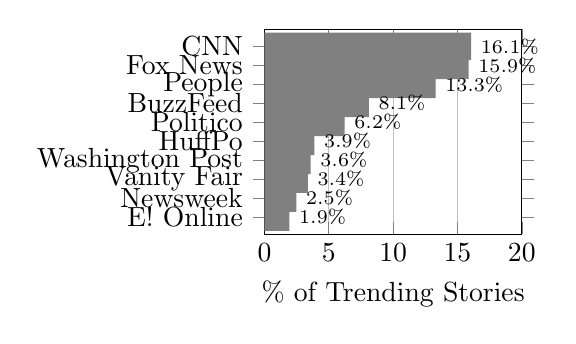
\begin{tikzpicture}
\begin{axis}[ 
width=0.4\textwidth,
xbar, xmin=0, xmax=20,
xmajorgrids=true,
nodes near coords=\pgfmathprintnumber{\pgfplotspointmeta}\%,
every node near coord/.append style={font=\scriptsize},
nodes near coords style={/pgf/number format/.cd,fixed zerofill,precision=1},
xlabel={\% of Trending Stories},
symbolic y coords={%
{E! Online},
{Newsweek},
{Vanity Fair},
{Washington Post},
{HuffPo},
{Politico},
{BuzzFeed},
{People},
{Fox News},
{CNN} },
ytick=data,
]
\addplot [fill=gray,draw=none]
coordinates {
(16.062341,{CNN})
(15.8715013,{Fox News})
(13.2951654,{People})
(8.110687,{BuzzFeed})
(6.2340967,{Politico})
(3.8804071,{HuffPo})
(3.5941476,{Washington Post})
(3.3715013,{Vanity Fair})
(2.480916,{Newsweek})
(1.9402036,{E! Online})
};
\end{axis}
\end{tikzpicture}
\end{center}
\caption{Relative distribution of Trending Stories across top ten sources, March 9th to May 9th, 2019 (n=3,144)}\label{fig-trending_stories_distribution}
\end{figure}



\begin{figure}[!t]
\begin{center}
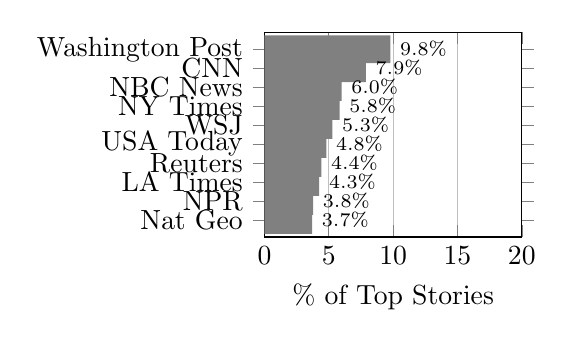
\begin{tikzpicture}
\begin{axis}[ 
width=0.4\textwidth,
xbar, xmin=0, xmax=20,
xlabel={\% of Top Stories},
xmajorgrids=true,
nodes near coords=\pgfmathprintnumber{\pgfplotspointmeta}\%,
every node near coord/.append style={font=\scriptsize},
nodes near coords style={/pgf/number format/.cd,fixed zerofill,precision=1},
symbolic y coords={%
{Nat Geo},
{NPR},
{LA Times},
{Reuters},
{USA Today},
{WSJ},
{NY Times},
{NBC News},
{CNN},
{Washington Post}
},
ytick=data,
]
\addplot [fill=gray,draw=none]
coordinates {
(9.7791798,{Washington Post})
(7.8864353,{CNN})
(5.9936909,{NBC News})
(5.8359621,{NY Times})
(5.2839117,{WSJ})
(4.8107256,{USA Today})
(4.4164038,{Reuters})
(4.2586751,{LA Times})
(3.785489,{NPR})
(3.7066246,{Nat Geo})
};
\end{axis}
\end{tikzpicture}
\end{center}
\caption{Relative distribution of Top Stories across top ten sources, March 9th to May 9th, 2019 (n=1,268)}\label{fig-top_stories_distribution}
\end{figure}

A key finding from our content analysis is the high concentration of sources in the algorithmically-curated Trending Stories section. Of the 83 unique sources observed in Trending Stories, CNN was the most common, with 505 unique stories (16.1\%) in the collection. The distribution across sources of Trending Stories was also highly skewed, as the three most common sources accounted for 1,422 stories (45.2\%). In contrast, out of 87 unique sources observed in Top Stories, the most common source accounted for 124 unique stories (9.8\%), and the three most common sources accounted for 300 stories (23.7\%). Across sections 40 sources appeared in both. While the Trending Stories achieved a Shannon equitability index of 0.689, the Top Stories achieved an index of 0.780. The Shannon indices indicate a significant difference (Hutcheson's t = 11.17, p < 0.001) in the diversity and evenness of sources between Top Stories and Trending Stories, as can be visualized in Figures \ref{fig-trending_stories_distribution} and \ref{fig-top_stories_distribution}. See Table \ref{summary-table} for a further comparison of source prominence and source diversity. 




% Time of first appearance - trending stories
\pgfplotstableread[row sep=\\,col sep=&]{
hour & pct   \\
0     & 4.2302799   \\
1     & 3.8804071   \\
2    & 3.5941476   \\
3   & 3.148855   \\
4   & 3.0534351   \\
5   & 3.8486005   \\
6   & 4.1666667   \\
7     & 4.7391858   \\
8     &  5.0572519   \\
9    & 5.8206107   \\
10   &  5.8206107   \\
11   &  4.1666667   \\
12   &  4.1030534   \\
13     &  3.6259542   \\
14    &  4.3256997   \\
15   & 3.8486005   \\
16   &  3.6895674   \\
17     &  4.1030534   \\
18     &  3.9122137   \\
19    &  3.7849873   \\
20   &  4.5483461   \\
21   &  3.8167939   \\
22   &  4.0076336   \\
23   &  4.7073791   \\
}\myhrdata
    
    
    
    
    
    
\begin{figure}[t]
\begin{center}
\begin{tikzpicture}
    \begin{axis}[
            ybar,
            ymajorgrids=true,
            enlargelimits=false,
            ymin=0,ymax=15,
            yticklabel=$\pgfmathprintnumber{\tick}$\%,
            bar width=0.5,
            xlabel={Hour of Day (PDT)},
            enlarge y limits={0.0,upper},
            enlarge x limits={0.04},
            height=0.2\textwidth,
            width=0.5\textwidth,
            xtick distance=4,
            ]
        \addplot[fill=gray,draw=none] table[x=hour,y=pct]{\myhrdata};
    \end{axis}
\end{tikzpicture}
\end{center}
\caption{Relative distribution of Trending Stories over the hours when they first appeared. New stories appear consistently throughout the day, peaking slightly at around 10am.}\label{fig-trending-stories-appearance-times}
\end{figure}


% Time of first appearance - top stories
\pgfplotstableread[row sep=\\,col sep=&]{
hour & pct   \\
0     & 4.2586751 \\
1     & 1.0252366   \\
2    & 0.7097792   \\
3   & 0.4731861   \\
4   & 0   \\
5   & 0.4731861   \\
6   & 1.340694   \\
7     & 7.2555205   \\
8     &  5.4416404   \\
9    & 4.1798107   \\
10   &  5.7570978   \\
11   &  2.681388   \\
12   &  1.1829653   \\
13     &  2.8391167   \\
14    &  13.4069401   \\
15   & 5.4416404   \\
16   &  3.5488959   \\
17     &  1.4195584   \\
18     &  2.9968454   \\
19    &  13.6435331   \\
20   &  6.1514196   \\
21   &  2.5236593   \\
22   &  2.0504732   \\
23   &  11.1987382   \\
}\myhrdata
    
\begin{figure}[t]
\begin{center}
\begin{tikzpicture}
    \begin{axis}[
            ybar,
            ymajorgrids=true,
            bar width=0.5,
            enlarge y limits={0.0,upper},
            enlarge x limits={0.04},
            ymin=0,ymax=15,
            xlabel={Hour of Day (PDT)},
            yticklabel=$\pgfmathprintnumber{\tick}$\%,
            height=0.2\textwidth,
            width=0.5\textwidth,
            xtick distance=4,
        ]
        \addplot[fill=gray,draw=none] table[x=hour,y=pct]{\myhrdata};
    \end{axis}
\end{tikzpicture}
\end{center}
\caption{Relative distribution of Top Stories over the hours when they first appeared. New stories appear more commonly at specific times in the day, such as 2pm or 7pm. }\label{fig-top-stories-appearance-times}
\end{figure}

\subsubsection{Update Patterns in Trending Stories vs. Top Stories}
Data from the extended collection suggests that Trending Stories follow a fairly consistent churn rate, with stories gradually trickling in throughout the day, while the Top Stories section receives punctuated updates in the morning, mid-day, afternoon, and evening. These update schedules are visualized in Figures \ref{fig-trending-stories-appearance-times} and \ref{fig-top-stories-appearance-times}.
\begin{comment}
This finding is consistent with the description in \citep{Nicas2018} of how Apple's staff updates the Top Stories: ``The lineup typically shifts five or more times a day, depending on the news. A single editor in London typically chooses the first mix of stories for the East Coast’s morning commute before editors in New York and then Cupertino step in.''
\end{comment}

\subsubsection{Topics in Trending Stories vs. Top Stories}
Our n--gram analysis highlights topical distinctions between the app's editorially-curated content and algorithmically-curated content. For example, the Trending Stories (see Table \ref{trending-only-ngrams}) frequently featured many celebrities (Lori Loughin, Kate Middleton, Justin Bieber, Olivia Jade, Stephen Colbert, Kim Kardashian), as well as some politicians (Donald Trump, Alexandria Ocasio-Cortez). Ocasio-Cortez never appeared in Top Stories, suggesting a mismatch between her trending popularity and the interests of editors; however, Trump appeared in both lists, indicating popularity-driven interest as evidenced by his full name trending, and also editorial interest in his activities as president of the United States. The Trending Stories section tended to feature more news that might be considered surprising, shocking, or sensational, with frequent terms such as ``found dead'' and ``florida man'' (referencing an Internet meme about Florida's purported notoriety for strange and unusual events\footnote{https://en.wikipedia.org/wiki/Florida\_Man}). On the other hand, the salient terms found in Top Stories (see Table \ref{top-only-ngrams}) featured more substantive policy issues related to topics like health care (e.g. ``affordable care act''), immigration (e.g. ``border wall'' and ``sanctuary city''), and international politicians and events (e.g. ``Kim Jong Un'' and ``brexit deal'') which never appeared in the Trending Stories headlines. Also, salient n--grams from Top Stories reflect news roundups which the editors feature regularly (e.g. ''biggest news'' and ``week's good news''), as well as some entertainment news (e.g. ''Avengers: Endgame'').


\begin{table}[!t]
\small
    \begin{subtable}{0.25 \textwidth}
      \centering
        \caption{Trending Stories}
        \begin{tabular}{@{}ll@{}}
            \toprule
            N--gram    & n \\
            \midrule
donald trump     & 65     \\
fox news     & 29     \\
donald trump's     & 25     \\
lori loughlin's     & 18     \\
kate middleton     & 16     \\
justin bieber     & 14    \\
found dead     & 13     \\
olivia jade     & 13      \\
alexandria ocasio-cortez     & 12     \\
prince william     & 12       \\
trump jr    & 12      \\
meghan markle     & 33*      \\
florida man     & 11     \\
ivanka trump     & 11      \\
jared kushner     & 11       \\
kim kardashian     & 11       \\
south carolina     & 11      \\
stephen colbert     & 11      \\
things that'll     & 11     \\
tucker carlson     & 11     \\

            \bottomrule
            \end{tabular}
    \label{trending-only-ngrams}
    \end{subtable}%
    \begin{subtable}{0.25 \textwidth}
      \centering
        \caption{Top Stories}
        \begin{tabular}{@{}ll@{}}
            \toprule
            N--gram    & n \\
            \midrule
    biggest news        & 9    \\
    measles cases        & 9    \\
    `sanctuary cities'        & 8    \\
    attorney general barr        & 8    \\
    affordable care act       & 7    \\
    trump threatens      & 7     \\
    2020 presidential      & 6   \\
    avengers: endgame       & 6    \\
    house panel       & 6    \\
    new zealand mosque       & 6    \\
    notredame fire       & 6    \\
    trump tax returns       & 6    \\
    week's good news       & 6    \\
    attorney general        & 16*    \\
    border wall        & 5    \\
    brexit deal        & 5    \\
    ground boeing 737        & 5    \\
    julian assange        & 5    \\
    kim jong un        & 5    \\
    timmothy pitzen        & 5    \\
            \bottomrule
            \end{tabular}
        \label{top-only-ngrams}
    \end{subtable} 
        \caption{The twenty most-salient n--grams in Trending Stories and Top Stories (as measured by the log ratio of occurences in each section's headlines), and the raw number of occurrences. In almost all cases, n--grams were unique to the section. Otherwise, n* indicates the n--gram appeared twice in the other section.}
\end{table}




\begin{table}[h]
\resizebox{0.47 \textwidth}{!}{
\begin{tabular}{@{}lll@{}}
\toprule
                    & Trending Stories & Top Stories \\ \midrule
Curation            & Algorithmic                 & Editorial          \\
Stories Displayed &  6 (4 on small screens)   &  5 \\
Localization        & National                    & National               \\
Personalization     & No                        &     No                  \\
Total Stories Analyzed & 3,144 & 1,267 \\

\midrule
Avg. Story Duration &  2.9hrs & 7.2hrs  \\

Avg. Stories per Day  &   50.7  &  20.4     \\   

Avg. Stories per Day per Slot  &   8.5  &  4.1   \\   
\midrule

Total Unique Sources & 83 & 87 \\

Shannon Equitability Index & 0.689 & 0.780 \\

Mean Source Share  &   1.2\%  &  1.1\%     \\   

Median Source Share  &   0.2\%  &  0.2\%     \\ 

Top Source Share      &    16.1\%      & 9.8\%          \\   

Top 3 Sources Share      &    45.2\%      & 23.7\%          \\   

Top 10 Sources Share      &    74.8\%      & 55.7\%          \\  
\bottomrule
\end{tabular}%

}
\caption{Summary of results. The top section focuses on high-level aspects, the middle on churn rate, and the lower on source distribution. ``Top N Source Share'' is defined as the percentage of stories that came from the N most common sources in the section.} \label{summary-table}
\end{table}